%Part of/Parte di https://github.com/f-dinucci/appuntiMeccanicaFluidi/
%License/Licenza Creative Commons Attribution-ShareAlike 4.0 International (CC BY-SA 4.0) - attribution/attribuzione Francesco Di Nucci
%See also/Vedere anche https://creativecommons.org/licenses/by-sa/4.0/ and/e https://creativecommons.org/licenses/by-sa/4.0/legalcode
%
\section{Teoria della lubrificazione}
\subsection{Teoria della lubrificazione di Reynolds}
La teoria della lubrificazione è un esempio di applicazione di flusso lentamente variabile e trova uso quando c'è necessità di separare due organi meccanici in moto relativo tra loro.
È una variante del problema di Couette, si hanno due lastre, di cui una inclinata.
Il moto del fluido fa nascere una forza ortogonale alle lastre, che tende a separarle.

Ci si pone nel sistema di riferimento della lastra superiore inclinata, anche detta pattino, in modo che il flusso sia stazionario.
In questo riferimento è la lastra inferiore (infinita) a muoversi.
%
	\begin{figure}[ht]
		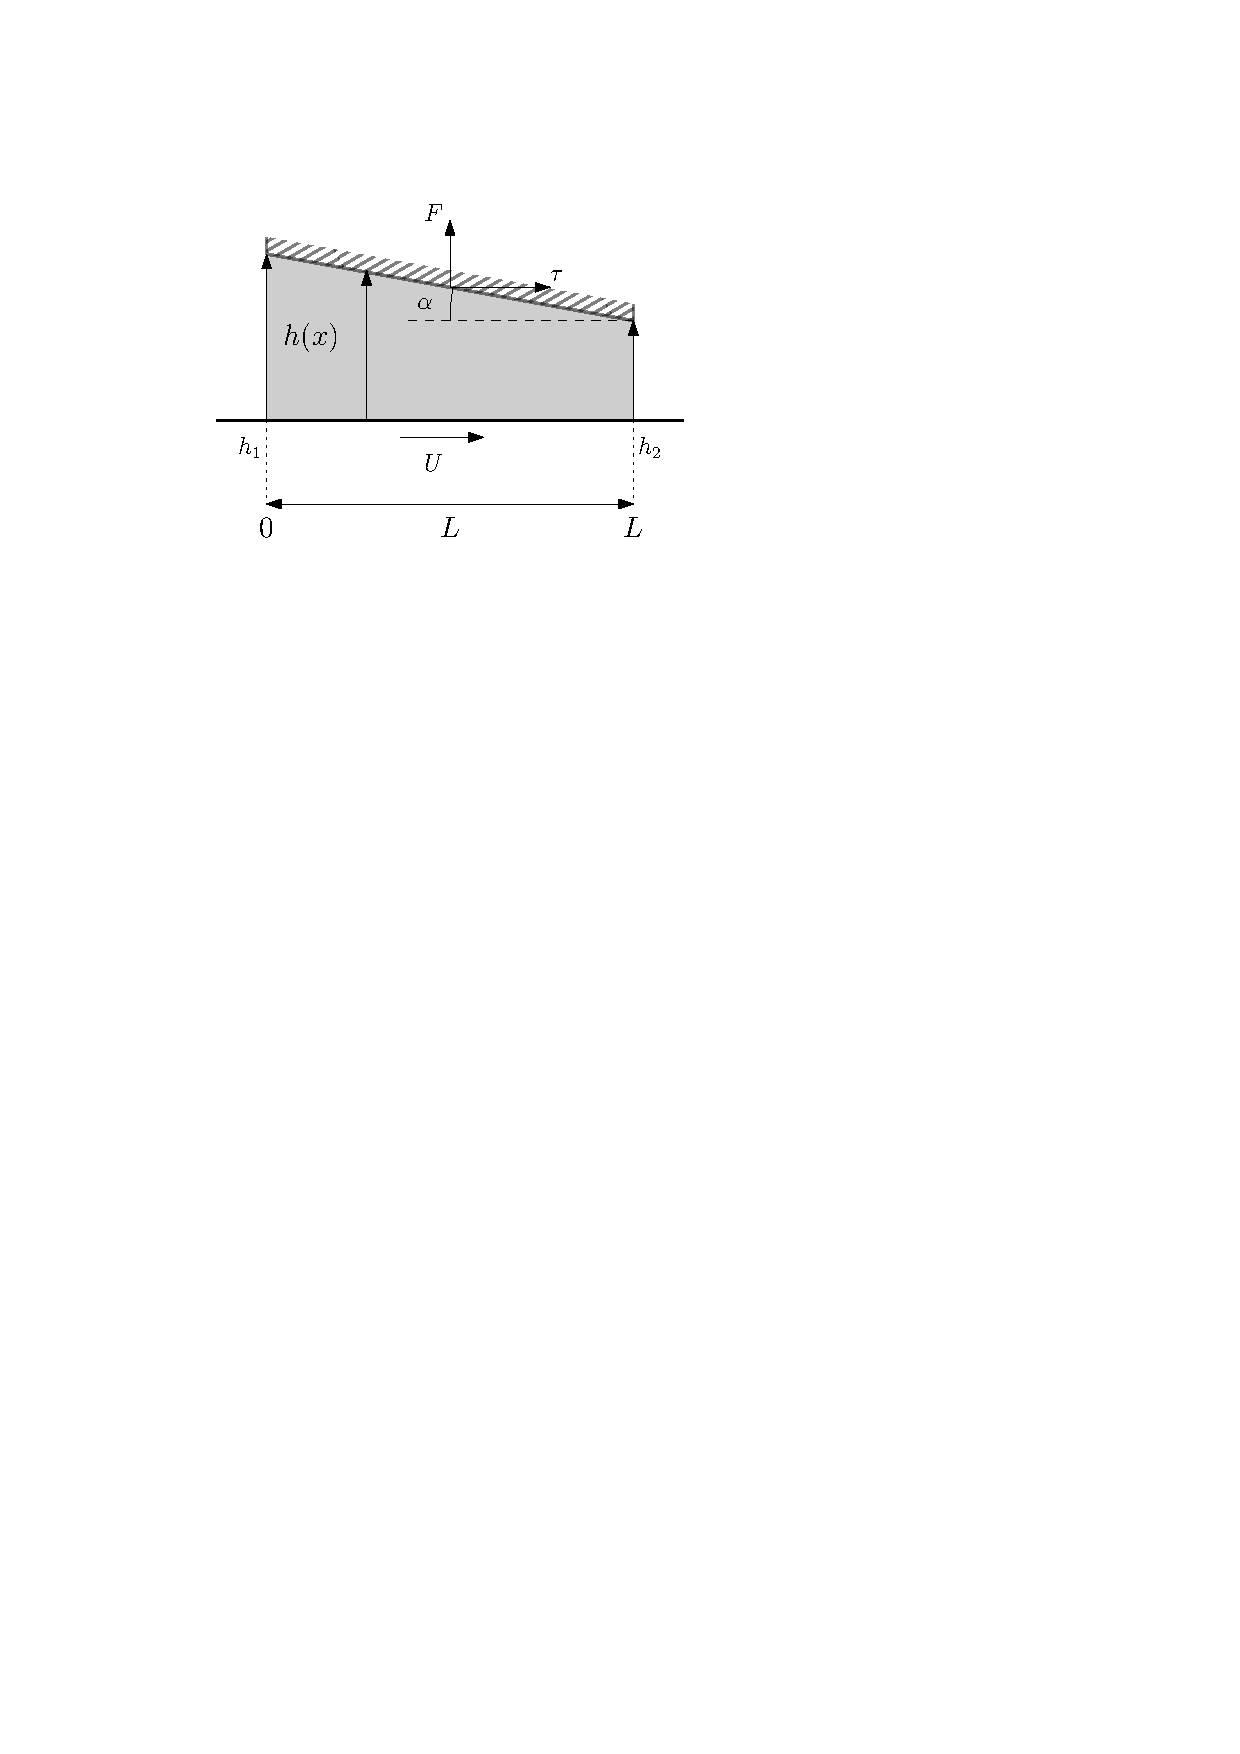
\includegraphics[scale=0.9]{./6.3 Teoria della lubrificazione/6.3-1}
		\centering
		\caption{Applicazione del flusso lentamente variabile}
	\end{figure}
%
Si suppone di avere lo stesso flusso del moto di Couette:
%
	\begin{equation*}
		u = U \left[ \frac{h(x) - y}{h(x)} \right]
	\end{equation*}
%
Quindi la portata sarebbe una $Q(x)$:
%
	\begin{equation*}
		Q = \int_o^h u \dd{y} = Q(x)
	\end{equation*}
%
Ma allo stesso tempo per l'equazione di continuità la portata deve essere la stessa per tutte le $x$:
%
	\begin{equation*}
		u_x + v_y = 0 \rightarrow \dv{x} \int_0^h u \dd{y} = 0
	\end{equation*}
%
Quindi non può essere un flusso di Couette, si vede che è invece un moto composto, flusso di Couette-Pouiseuille:
%
	\begin{equation*}
		u = U \frac{h - y}{h} - \frac{p_x}{2 \mu} y (h - y)\\
	\end{equation*}
%
La portata contiene quindi $p_x$ come incognita, che può essere usata come condizione per imporre la portata costante, rimane solamente $h(x)$ variabile:
%
	\begin{equation*}
		\begin{gathered}
			Q = \int_0^h u \dd{y} = U \frac{h}{2} - \frac{p_x}{12 \mu} h^3\\
			p_x = 12 \mu \left( \frac{U}{2 h^2} - \frac{Q}{h^3} \right)
		\end{gathered}
	\end{equation*}
%
Si impongono poi le condizioni al contorno, sia all'ingresso che all'uscita il fluido è in equilibrio con l'atmosfera, quindi la pressione è uguale a quella atmosferica:
%
	\begin{equation*}
		p(0) = p(L) = p_0
	\end{equation*}
%
Dato che che la pressione di ingresso è uguale a quella di uscita, si ha che:
%
	\begin{equation*}
		\begin{gathered}
			p(x) = p_0 + \int_0^h p_x \dd{x} = p_0 + \int_0^x 12 \mu \left( \frac{U}{2 h^2(x)} - \frac{Q}{h^3(x)} \right) \dd{x}\\
			\int_0^L \left( \frac{U}{2 h^2(x)} - \frac{Q}{h^3(x)} \right) \dd{x} = 0\\
			Q = U \frac{\int_0^L \frac{1}{2 h^2} \dd{x} }{\int_0^L \frac{1}{h^3} \dd{x}}
		\end{gathered}
	\end{equation*}
%
Nota la portata, si possono ricavare pressione e velocità.
La pressione ha un andamento come nel grafico seguente e genera una forza:
%
	\begin{equation*}
		F = \int_0^L p \dd{x} >0
	\end{equation*}
%
%
	\begin{figure}[ht]
		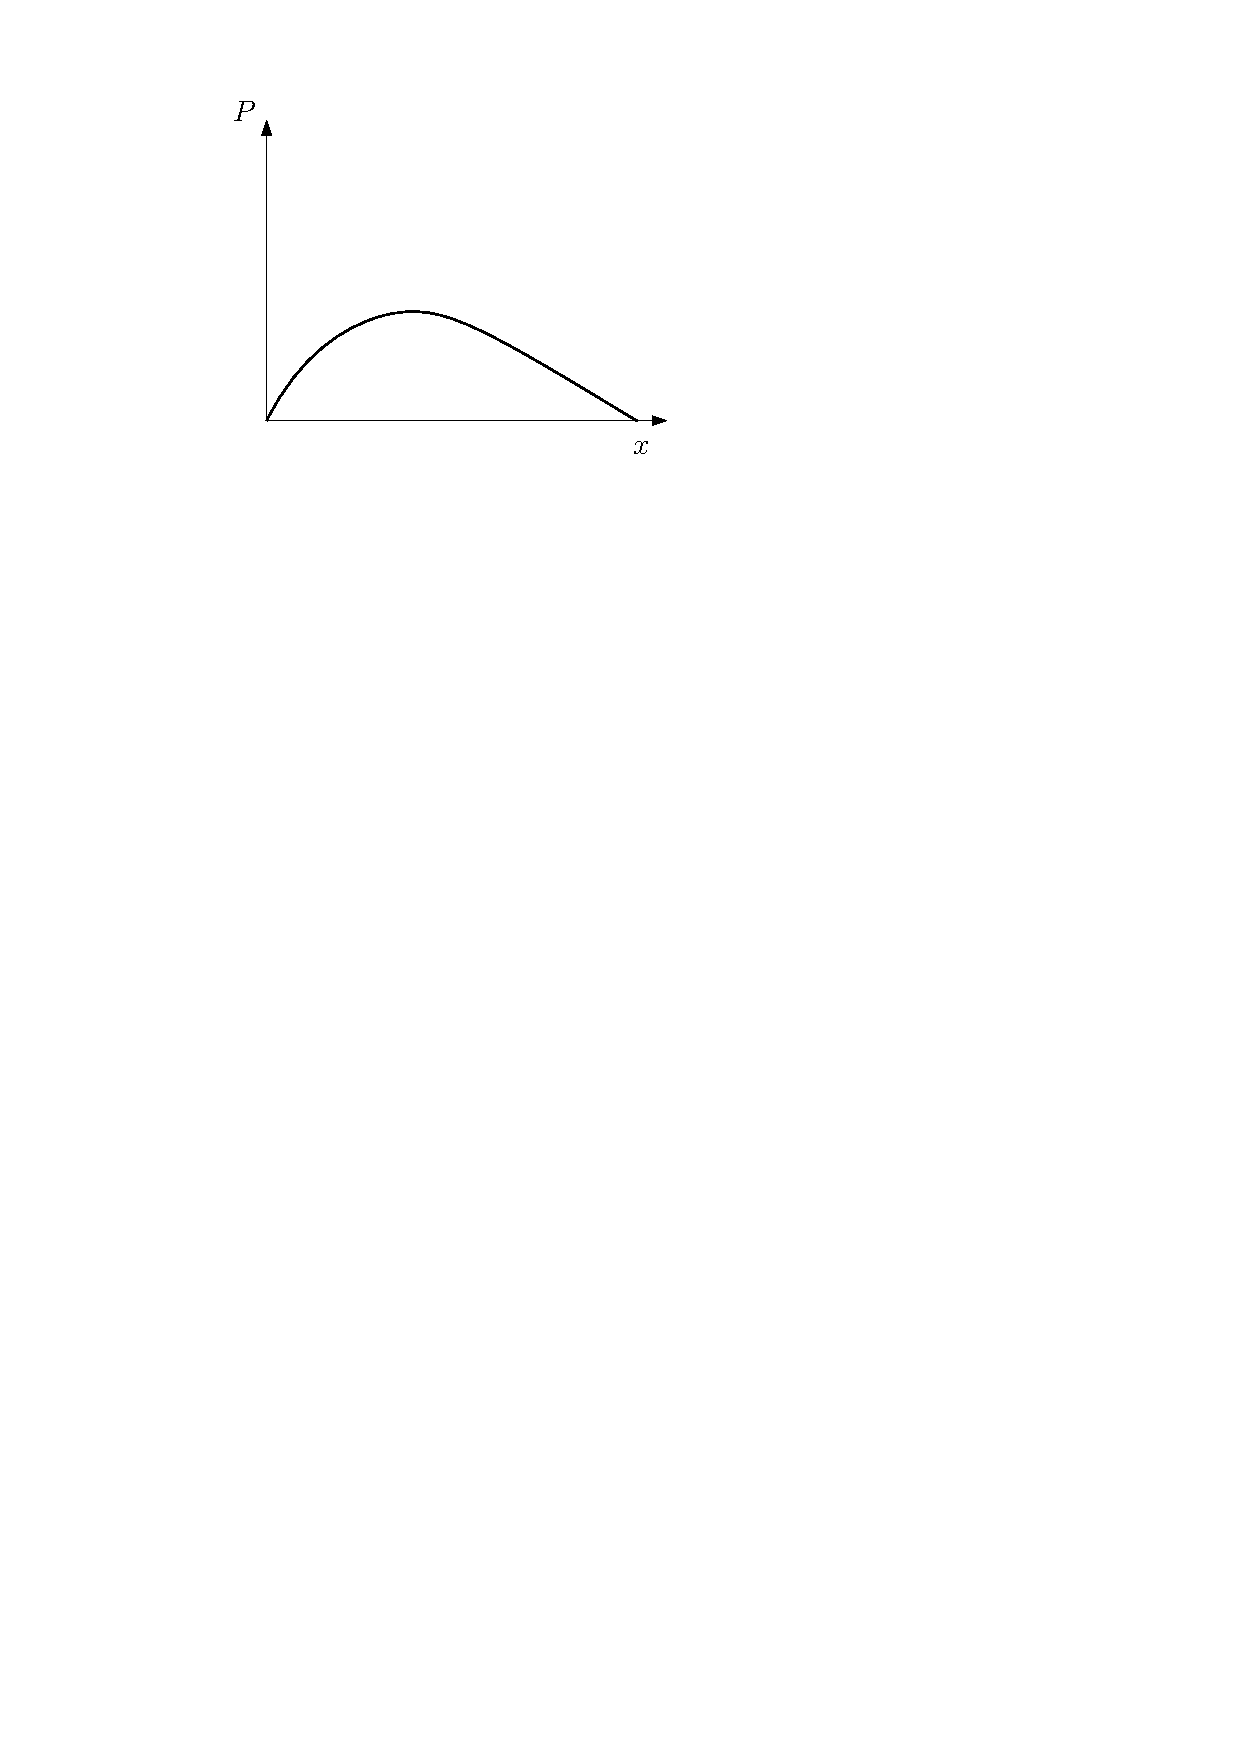
\includegraphics[scale=0.7]{./6.3 Teoria della lubrificazione/6.3-2}
		\centering
		\caption{Andamento della pressione relativa}
	\end{figure}
%
Questo è il principio alla base della lubrificazione, si genera una forza che separa i due componenti in moto tra loro (che più è grande quanto $\frac{h}{L}$ è piccolo) quindi ad un certo punto la distanza tra i due componenti si stabilizzerà.
La forza risultante è nulla nel caso in cui $\alpha = 0$, dal quale risulta $p = p_{atm}$, che in pratica riporta al caso del flusso di Couette.

Gli ordini di grandezza sono:
%
	\begin{equation*}
		\begin{gathered}
			p_x \sim 12 \mu \frac{U}{h^2}\\
			p \sim 12 \mu \frac{U}{h^2} L\\
			F_y \sim 12 \mu U \frac{L^2}{h^2}
		\end{gathered}
	\end{equation*}
%
Ovviamente c'è anche una componente orizzontale della forza (che si avrebbe anche per $\alpha = 0$):
%
	\begin{equation*}
		\begin{gathered}
			\tau = \mu \left( - \frac{U}{h} + h \frac{p_x}{2 \mu} \right)\\
			\text{ordine di grandezza}\\
			\tau \sim \mu \frac{U}{h}\\
			F_x = \int \tau \dd{x} \sim \mu U \frac{L}{h}
		\end{gathered}
	\end{equation*}
%
Il rapporto tra le due componenti della forza dà il coefficiente d'attrito tra solidi, dato che per organi meccanici si vuole una piccola forza tangenziale per una data forza normale, tramite modifiche alla geometria si può entro certi limiti legati alla rugosità controllare l'attrito:		
%
	\begin{equation*}
		\frac{F_x}{F_y} \sim \frac{h}{L}
	\end{equation*}
%

\subsection*{Bibliografia 6.3}
\cite[Cap.\ 9.2]{PnueliGutfinger}